\documentclass[10pt, compress]{beamer}

\usetheme{metropolis}
\usepackage{appendixnumberbeamer}

\usepackage{tikz-dependency}
\usepackage{caption}
\usepackage{polyglossia}
\usepackage{booktabs}
\usepackage{tabularx}
\usepackage{alltt}
\usepackage{framed}
\usepackage[scale=2]{ccicons}

\usepackage{pgfplots}
\usepgfplotslibrary{dateplot}

\usepackage{xspace}
\newcommand{\themename}{\textbf{\textsc{metropolis}}\xspace}

% commands from the paper
%\setmainfont[Scale=1.0]{Fira Sans Light}

\newfontfamily\gtfont[Scale=1.1,Letters=SmallCaps]{Linux Libertine O}
\newcommand{\udtag}[1]{{\ll \textsc{#1}}}
\newcommand{\gtlabel}[1]{{\gtfont #1}}
\newcommand{\udlabel}[1]{{\tt #1}}
\newfontfamily\udfont[Scale=0.9,Letters=SmallCaps]{Linux Libertine O}
\newcommand{\utag}[1]{{\udfont#1}}
\newcommand{\ufeat}[1]{{\udfont#1}}
\newcommand{\tgl}[1]{{\em #1}}
\setmonofont[Scale=MatchLowercase]{DejaVu Sans Mono}

% commands from the paper


\newcommand{\myarrow}[1][-45]{%
  \mathrel{%
    \text{$
     \begin{tikzpicture}[baseline = -0.5ex]
       \node[inner sep=0pt,outer sep=0pt,rotate = #1] (a) at (0,0)  {$\xrightarrow{}$};
    \end{tikzpicture}
    $}%
  }%
}%




\title{Class 05: Named-entity recognition}

\begin{document}

\maketitle

\begin{frame}{Information extraction}

\begin{center}
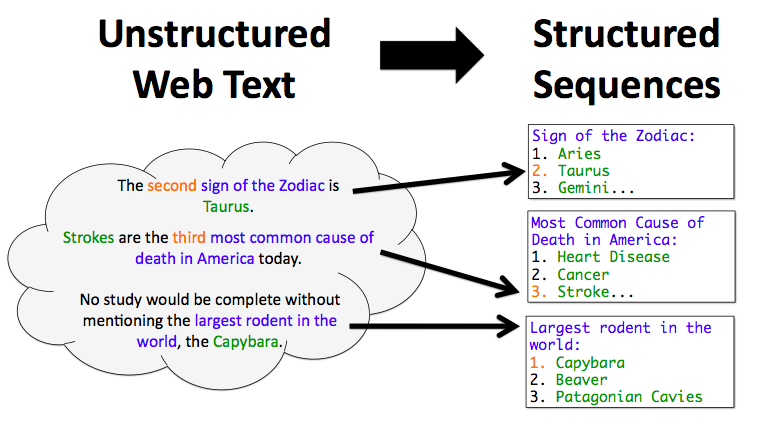
\includegraphics[width=0.8\textwidth]{graphics/inform-extract.png}
\end{center}

% background

\begin{itemize}
  \item Take unstructured text and produce structured data
  \item Used in question answering 
\end{itemize}

\begin{center}
``Who is the president of Finland?''
\end{center}

\end{frame}


\begin{frame}{Named-entity recognition}

\begin{onlyenv}<1>
\begin{framed}
Саули Вяйнямё Нийнистё (24 августа 1948 года, Сало, Финляндия) — финский 
государственный деятель, политик, юрист, действующий президент Финляндии с 1 марта 2012 года. 
\end{framed}
\end{onlyenv}
\begin{onlyenv}<2>
\begin{framed}
\alert<2>{[PER Саули Вяйнямё Нийнистё]} (24 августа 1948 года, \alert<2>{[LOC Сало], [LOC Финляндия]}) — финский 
государственный деятель, политик, юрист, действующий президент \alert<2>{[LOC Финляндии]} с 1 марта 2012 года. 
\end{framed}
\end{onlyenv}

\begin{itemize}
  \item First step in information extraction
  \item Find each mention of a \textbf{named entity} and label it with \textbf{type}
\end{itemize}


\end{frame}

\begin{frame}{Named-entity types}

\begin{onlyenv}<1>
\vspace{60pt}
\begin{tabular}{llll}
  \textbf{Type} & \textbf{Tag} & \textbf{Categories} & \\
  People & {\sc per} & people, characters & \\
  Organisation & {\sc org} & companies, teams & \\
  Location & {\sc loc} & regions, mountains, seas & \\
  Geopolitical entity & {\sc gpe} & countries, states, provinces & \\
  Facility & {\sc fac} & bridges, airports, buildings & \\
  Vehicles & {\sc veh} & planes, trains, cars & \\
\end{tabular}
\end{onlyenv}
\begin{onlyenv}<2->
\begin{center}
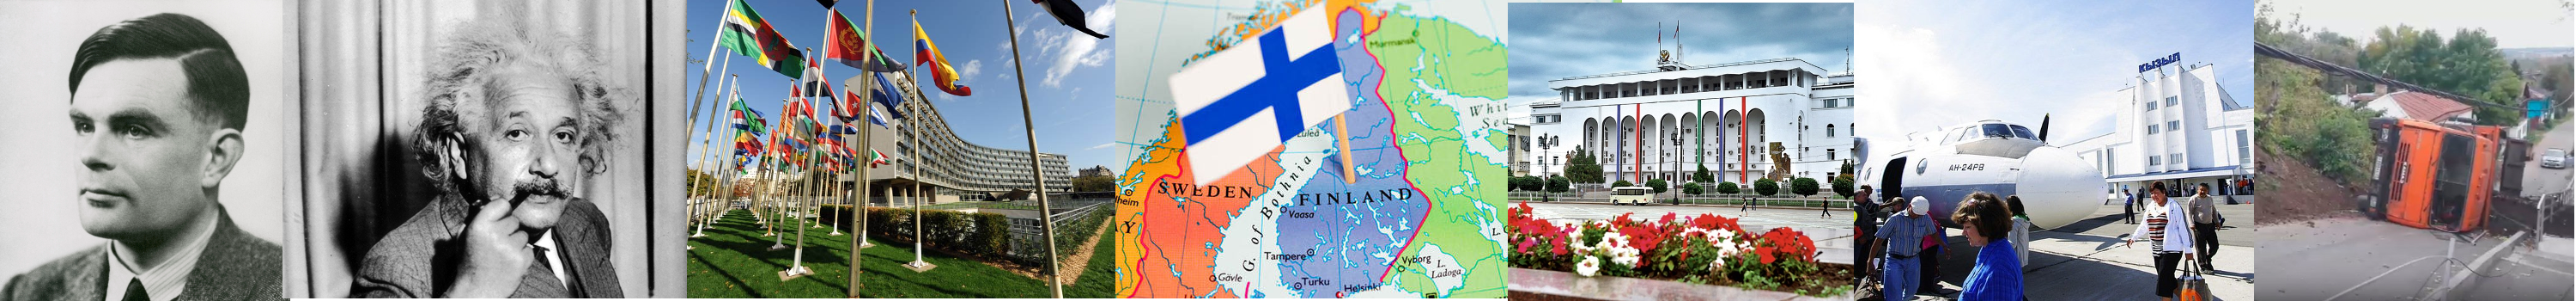
\includegraphics[width=\textwidth]{graphics/ner-banner.png}
\end{center}
\begin{tabular}{rl}
  \textbf{Tag} & \textbf{Example} \\
  {\sc per} & В возрасте 16 лет, \alert<3>{Тьюринг} ознакомился с работой \alert<3>{Эйнштейна}. \\
  {\sc org} & Бюджет \alert<3>{ЮНЕСКО} утверждается каждые два года. \\
  {\sc loc} & А прчему б в \alert<3>{Финляндию} не поехать? \\
  {\sc gpe} & \alert<3>{Дагестан} получит поддержку из федерального бюджета. \\
  {\sc fac} & В \alert<3>{аэропорту Кызыла} пройдет реконструкция. \\
  {\sc veh} & В центре Владимира перевернулся \alert<3>{КАМАЗ} с землёй. \\
\end{tabular}
\end{onlyenv}

\end{frame}

\begin{frame}{Ambiguity/1}

\begin{center}
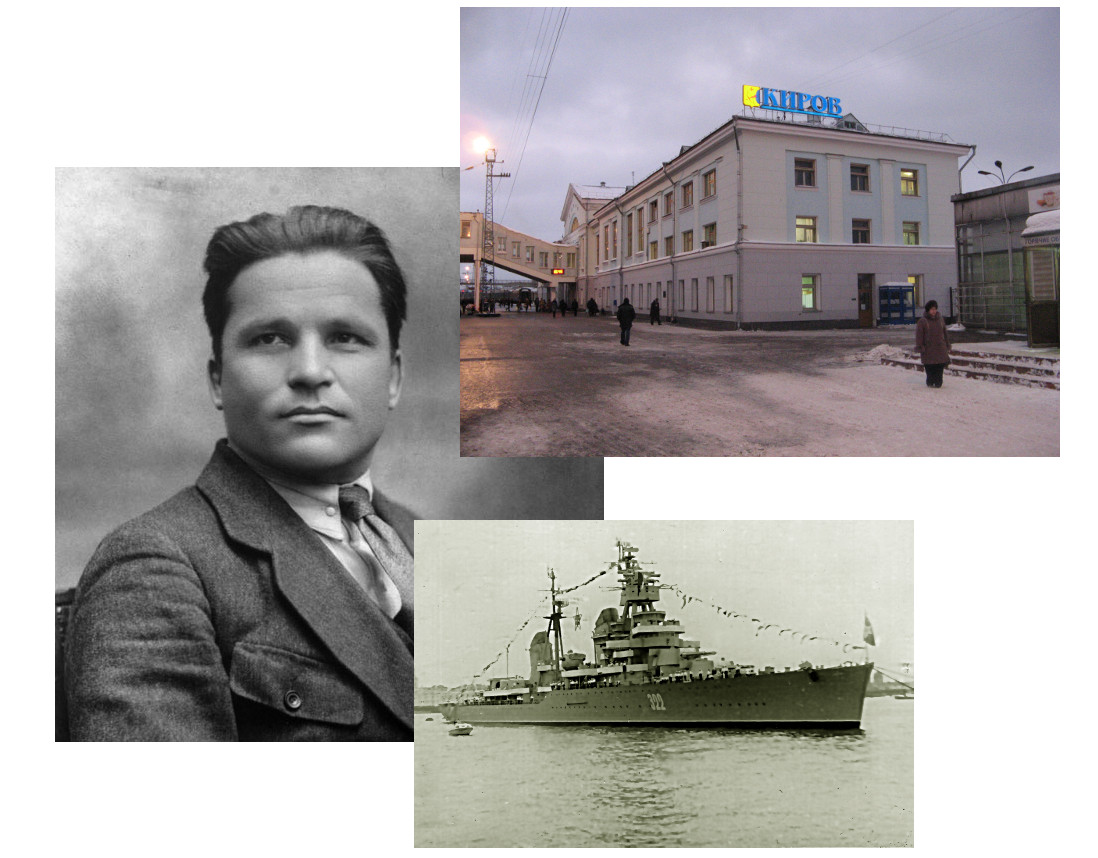
\includegraphics[width=0.65\textwidth]{graphics/kirov-all.jpg}
\end{center}

5 декабря 1934 года в память о [{\sc per} С. М. Кирове] президиум [{\sc org} ВЦИК] принял постановление о переименовании города [{\sc loc} Вятки] в город [{\sc loc} Киров] и образовании [{\sc loc} Кировского края], с центром в городе [{\sc loc} Кирове].

\end{frame}

\begin{frame}{Ambiguity/2}

\begin{itemize}
\item 5 декабря 1934 года в память о [{\sc per} С. М. Кирове] президиум [{\sc org} ВЦИК] принял постановление о переименовании города [{\sc loc} Вятки] в город [{\sc loc} Киров] и образовании [{\sc loc} Кировского края], с центром в городе [{\sc loc} Кирове].
~\\
~\\
\item 5 декабря 1934 года в память о [{\sc per} С. М. Кирове] [{\sc org} \alert<2>{президиум} ВЦИК] принял постановление о переименовании [{\sc loc} \alert<2>{города} Вятки] в [{\sc loc} \alert<2>{город} Киров] и образовании [{\sc loc} Кировского края], с центром в [{\sc loc} \alert<2>{городе} Кирове].
\end{itemize}

\end{frame}



\begin{frame}{Sequence labelling}

~\\

\begin{columns}
\begin{column}{0.48\textwidth}
Typical classifiers:
\begin{itemize}
\item CRF
\item MEMM
\end{itemize}

Each token gets a label:
\begin{itemize}
\item [{\tt B}] Begin NE + type
\item [{\tt I}] Inside NE + type
\item [{\tt O}] Outside NE + type
\end{itemize}
\end{column}
\begin{column}{0.48\textwidth}
{\small 
\begin{tabular}{lll}
\textbf{Word} & \textbf{BIO label} \\
\hline
Доклад & {\tt O} \\
директора & {\tt O} \\
федерального & {\tt O} \\
Института & {\tt B-ORG} \\
национальных & {\tt I-ORG} \\
школ & {\tt I-ORG} \\
Светланы & {\tt B-PER} \\
Семёновой & {\tt I-PER} \\
был & {\tt O} \\
посвящён & {\tt O} \\
изучению & {\tt O} \\
якутского & {\tt O} \\
языка & {\tt O} \\
на & {\tt O} \\
современном & {\tt O} \\
этапе & {\tt O} \\
. & {\tt O} \\
\end{tabular}
}
\end{column}

\end{columns}
\end{frame}

%\begin{frame}{Example}

%\end{frame}


\begin{frame}{Typical features/1}

\begin{tabular}{ll}
identity of $w_i$  &  \\
identity of neighbouring words  &  \\
part of speech of $w_i$  &  \\
part of speech of neighbouring words  &  \\
presence of $w_i$ in a \emph{gazetteer} &  \\
$w_i$ is all uppercase &  \\
prefix of $w_i$ for length $\le 4$ &  \\
suffix of $w_i$ for length $\le 4$ &  \\
word shape of $w_i$ &  \\
word shape of neighbouring words &  \\
short word shape of $w_i$ \\
short word shape of neighbouring words &  \\
presence of hyphen &  \\

\end{tabular}

\end{frame}

\begin{frame}{Typical features/1}

\begin{tabular}{ll}
\textbf{Feature} & \textbf{Value} \\ 
identity of $w_i$  & Роскомнадзор \\
$w_i$ is all uppercase & False \\
prefix of $w_i$ & Р \\
prefix of $w_i$ & Ро \\
prefix of $w_i$ & Рос \\
prefix of $w_i$ & Роск \\
suffix of $w_i$ & дзор \\
suffix of $w_i$ & зор \\
suffix of $w_i$ & ор \\
suffix of $w_i$ & р \\
word shape of $w_i$ & Xxxxxxxxxxxx \\
short word shape of $w_i$ & Xx \\
presence of hyphen & False  \\

\end{tabular}

\end{frame}

\begin{frame}{Gazetteers (рус. Географический справочник)}

What are gazetteers?
\begin{itemize}
  \item List of place names 
  \item Can include millions of entries
  \item Also other information (population size, etc.)
\end{itemize}

Similarly, lists can be found of:
\begin{itemize}
  \item Person names (e.g. ФИО)
  \item Corporations
  \item Product names
\end{itemize}

Usefulness varies depending on the class of named entity.

% A gazetteer is a list of place names, and they can offer millions of entries for gazetteer
% all  manner  of  locations  along  with  detailed  geographical,  geologic,  and  political
% information. In addition to gazeteers, the United States Census Bureau provides
% extensive lists of first names and surnames derived from its decadal census in the U.S.
% Similar lists of corporations, commercial products, and all manner of things
% biological and mineral are also available from a variety of sources. Gazeteer features
% are typically implemented as a binary feature for each name list. Unfortunately, such
% lists can be difficult to create and maintain, and their usefulness varies considerably
% depending on the named entity class.  It appears that gazetteers can be quite effec-
% tive, while extensive lists of persons and organizations are not nearly as beneficial
% (Mikheev et al., 1999)



\end{frame}

\begin{frame}{Domains}

\begin{center}
  
\includegraphics[width=\textwidth]{graphics/kfe-mak.png}
\end{center}

\begin{itemize}
  \item Effectiveness of features can vary by domain
  \item Features good for newswire text might not work for social media
  
\end{itemize}

\end{frame}


\begin{frame}{Evaluation}
%The familiar metrics of recall, precision, and F1 measure
%are used to evaluate NER systems.  Remember that recall is the ratio of the number of correctly labeled re-
%sponses to the total that should have been labeled; precision is the ratio of the num-
%ber of correctly labeled responses to the total labeled; and F -measure is the harmonic mean

Standard evaluation:
\begin{itemize}
  \item Precision 
  \item Recall 
  \item $F_1$
\end{itemize}

% The fact that named entity tagging has a segmentation component which is not
% present in tasks like text categorization or part-of-speech tagging causes some prob-
% lems with evaluation. For example, a system that labeled American but not American Airlines
% as an organization would cause two errors, a false positive for O and a false
% negative for I-ORG. In addition, using entities as the unit of response but words as
% the unit of training means that there is a mismatch between the training and test
% conditions.

% @@@ TODO @@@


\end{frame}

\begin{frame}{Producing training data}



\end{frame}

\begin{frame}{Manually annotated}

\begin{center}
  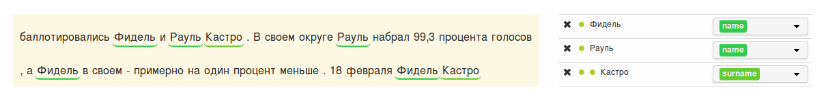
\includegraphics[width=0.9\textwidth]{graphics/factru-anno.png}
%  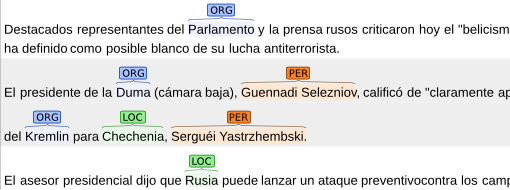
\includegraphics[width=0.9\textwidth]{graphics/esp.train-doc-536-small.png}
\end{center}

\end{frame}

\begin{frame}{Wikipedia/1}
% also manually annotated, kindof

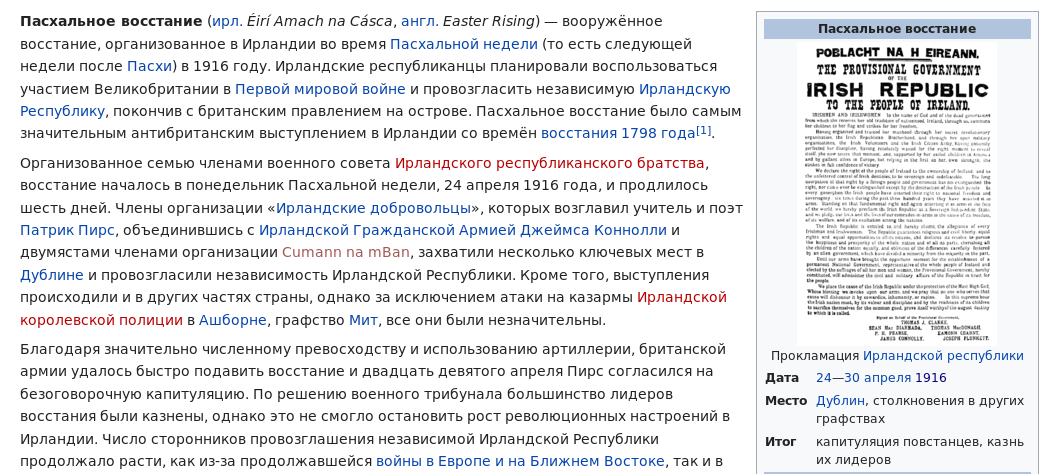
\includegraphics[width=\textwidth]{graphics/wikipedia-1.png}

\end{frame}

\begin{frame}{Wikipedia/2}

{\tt
Члены организации «[[Ирландские добровольцы]]», которых возглавил учитель 
и поэт [[Пирс, Патрик|Патрик Пирс]], объединившись с [[Ирландская гражданская армия|Ирландской Гражданской Армией]] [[Коннолли, Джеймс|Джеймса Коннолли]] и двумястами членами организации [[Совет ирландских женщин|Cumann na mBan]], захватили несколько ключевых мест в \alert<2>{[[Дублин]]е} и провозгласили независимость Ирландской Республики. 
}
\end{frame}

\begin{frame}{Wikipedia/3}
 % Cats

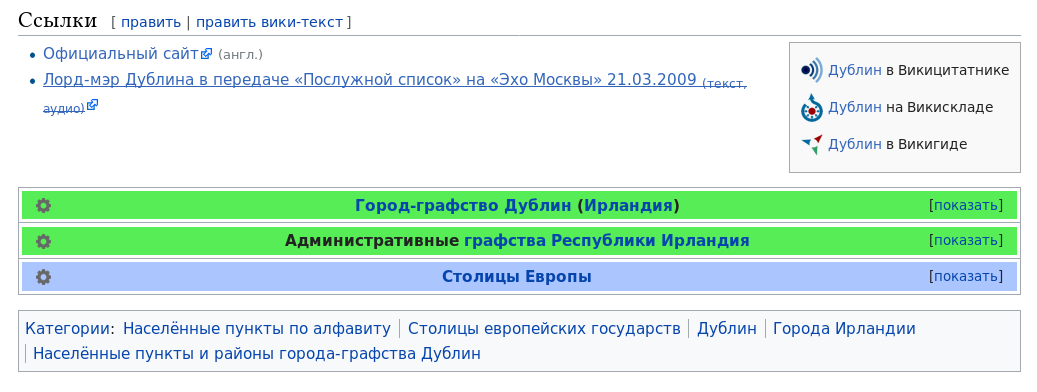
\includegraphics[width=\textwidth]{graphics/wikipedia-2.png}

\end{frame}

\begin{frame}{Wikipedia/4}

\begin{itemize}
\item \textbf{Ирландские добровольцы}
  \begin{itemize}
    \item История Ирландии; \alert<2>{Организации, основанные в 1913 году}; Ирландский национализм
  \end{itemize}
\item \textbf{Пирс, Патрик}
  \begin{itemize}
    \item \alert<2>{Персоналии по алфавиту}; Родившиеся 10 ноября; \alert<2>{Политики Ирландии}; \alert<2>{Революционеры Ирландии}; \ldots
  \end{itemize}
\item \textbf{Ирландская гражданская армия}
\begin{itemize}
  \item \alert<2>{Боевые организации политических партий}; Дублин; Ирландия; \alert<2>{Леворадикальные организации}
\end{itemize}
\item \textbf{Коннолли, Джеймс}
\begin{itemize}
  \item \alert<2>{Персоналии по алфавиту}; \alert<2>{Политики по алфавиту}; \alert<2>{Революционеры Ирландии}; \alert<2>{Синдикалисты}; \alert<2>{Эсперантисты}; \ldots
\end{itemize}
\item \textbf{Совет ирландских женщин}
\begin{itemize}
  \item Совет ирландских женщин; Ирландский национализм
\end{itemize}
\item \textbf{Дублин}
\begin{itemize}
  \item \alert<2>{Населённые пункты по алфавиту}; \alert<2>{Столицы европейских государств}; Дублин; \alert<2>{Города Ирландии}; \ldots
\end{itemize}
\end{itemize}

\end{frame}

\begin{frame}{Wikipedia/5}

{\tt
Члены организации «[{\sc ORG} Ирландские добровольцы]», которых возглавил 
учитель и поэт [{\sc PER} Патрик Пирс], объединившись с [{\sc ORG} Ирландской 
Гражданской Армией] [{\sc PER} Джеймса Коннолли] и двумястами членами 
организации \alert<2>{Cumann na mBan}, захватили несколько ключевых мест 
в [{\sc LOC} Дублине] и провозгласили независимость \alert<2>{Ирландской Республики}.
}

\end{frame}

\begin{frame}{Wikipedia/6}

\begin{itemize}
  \item Nothman, J. (2008) ``Transforming Wikipedia into Named Entity Training Data''. \emph{Proceedings of the Australasian Language Technology Association Workshop}
  \item Hahm, Y. et al. (2014) ``Named Entity Corpus Construction using Wikipedia and DBpedia Ontology''. \emph{LREC 2014}
  \item Сысоев, А. А. and Андрианов, И. А. (2016) ``Named entity recognition in Russian: The power of a Wiki-based approach''. \emph{Proceedings of the International Conference “Dialogue 2016”}
\end{itemize}

\end{frame}



\begin{frame}[standout]
Shared tasks
\end{frame}

\begin{frame}{CoNLL 2003}



\end{frame}

\begin{frame}{Data}

\begin{center}
\url{https://github.com/synalp/NER/tree/master/corpus/CoNLL-2003}
\end{center}

Form, Tag, Chunk, BIO label

\begin{alltt}

Australia NNP I-NP I-LOC  \\ 
will MD I-VP O \\ 
defend VB I-VP O \\ 
the DT I-NP O \\ 
Ashes NNP I-NP I-MISC \\ 
against IN I-PP O \\
England NNP I-NP I-LOC \\
during IN I-PP O \\ 
a DT I-NP O \\ 
four-month JJ I-NP O \\ 
tour NN I-NP O \\ 

\end{alltt}

\end{frame}

\begin{frame}{FactRuEval 2016}

\begin{itemize}
  \item Three tracks: Two for named entities and one for fact extraction
  \item First track (named entities) most popular
  \item Anonymous
\end{itemize}

\end{frame}

\begin{frame}{First track}

Classic named-entity recognition for Russian.

\end{frame}


\begin{frame}{Layered annotation model}


\end{frame}

\begin{frame}{Data}

\end{frame}

\begin{frame}{Participants}

\begin{center}
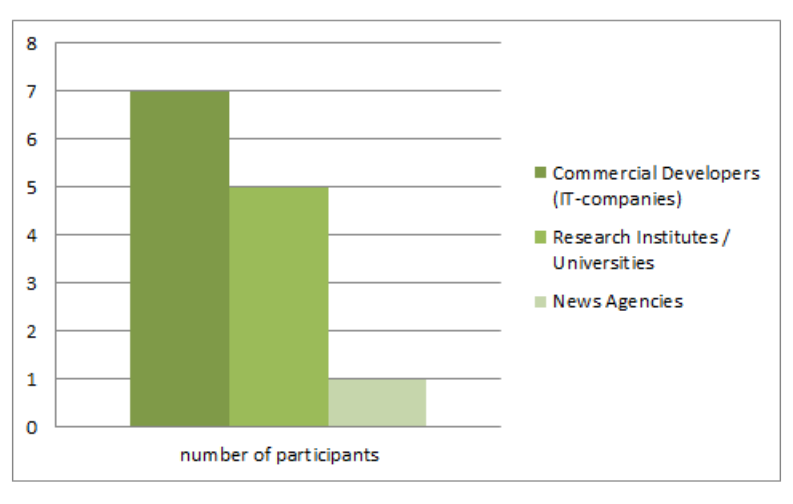
\includegraphics[width=\textwidth]{graphics/factrueval-participants.png}
\end{center}

\end{frame}

\begin{frame}{Results}

\begin{center}
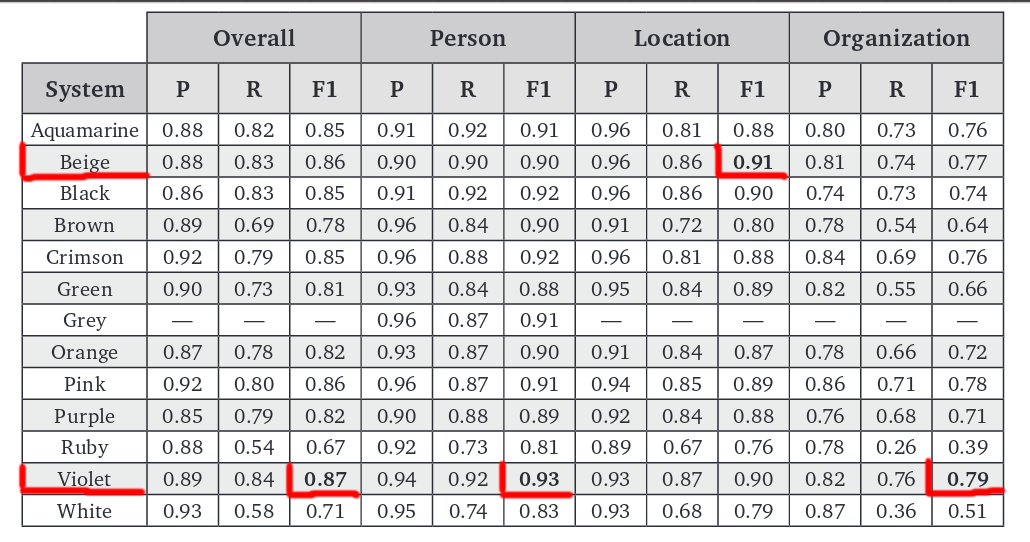
\includegraphics[width=\textwidth]{graphics/factrueval-results.png}
\end{center}

\begin{itemize}
  \item Similar performance to systems for English
\end{itemize}


\end{frame}

\begin{frame}[standout]
Practical
\end{frame}

\begin{frame}

\begin{itemize}
 \item Create a NER system for the CoNLL-2003 shared task for English using
   whatever classifier stuff you want
 \item Run a known NER system on the FactRuEval data
 \item Produce a corpus for NER using Wikipedia for a given language
\end{itemize}

\end{frame}



\end{document}
